\section{APPROACH}

The previous work presented a multi-robot exploration system that can efficiently explore unknown terrain, and is robust to robot failures. Our approach accomplishes the same using a strategy based on the market model. 
In this paper we determine the target points for each mobile robot in the team using an objective function which is a combination of frontier point cost, utility (information gain) and the frontier occupancy function. 

\subsection{Market-based strategy} 

At the core of our approach is negotiation between mobile robots during exploration. The mobile robots exchange information under the assumption of a fully connected graph, where all mobile robots communicate with each other and in the negotiation process each mobile robot takes into account the data received from all other mobile robots.

Every mobile robot $i$ gets the list of frontier points:

\begin{equation}
   \boldsymbol{y}=\begin{bmatrix}
    \boldsymbol{y_{0}} & \boldsymbol{y_{1}} & \boldsymbol{y_{2}} & \hdots & \boldsymbol{y_{M}}
\end{bmatrix},
\end{equation}

where $M$ is  the number of frontier points, and every list member is a vector consisting of the $x$ and $y$ coordinates. 

\begin{equation}
   \boldsymbol{y}=\begin{bmatrix}
   \begin{bmatrix}
           x_{0} \\
           y_{0} 
   \end{bmatrix}
    \begin{bmatrix}
         x_{1} \\
         y_{1} 
    \end{bmatrix}
    \begin{bmatrix}
         x_{2} \\
         y_{2} 
    \end{bmatrix}
    \hdots
    \begin{bmatrix}
         x_{M} \\
         y_{M} 
    \end{bmatrix}
\end{bmatrix}.
\end{equation}


We define the frontier point weight as a function of cost, utility and frontier occupancy. If $i$ is the index of the mobile robot, and $j$ is the index of the frontier point, then the cost function: $C_{ij}$: $R$ \(\rightarrow \text{$\mathbb{R}^{+}$}\) is a mapping from the set of resources $R$ to a positive real number. $C_{ij}$ describes the cost of $i$th robot to visit the $j$th frontier point. The cost can be a function of time, energy or, like in our case, the estimated distance travelled by mobile robot to reach the target frontier point. The estimated distance is approximated using Euclidean distance between the mobile robot position $\boldsymbol{p_{i}}$ and the frontier point position $\boldsymbol{q_{j}}$:

\begin{equation}\small
    C_{ij}=d(\boldsymbol{p_{i}}, \boldsymbol{q_{j}}) = \sqrt{(p_{ix}-q_{jx})^{2}+(p_{iy}-q_{jy})^{2}}.
    \label{cost}
\end{equation}

The utility function $U_{ij}$:  \(\text{$\mathcal {M}$}\) \(\rightarrow \text{$\mathbb{R}^{+}$}\) returns a positive real number from the occupancy grid \(\text{$\mathcal {M}$}\). The cells of \(\text{$\mathcal {M}$}\) may be marked as explored space, unexplored space or obstacle. The utility function is proportional to the number of the unexplored cells ($c$) within a fixed distance from the frontier point $j$ in the previous defined radius $r$: 

\begin{equation}
    U_{ij} = \lambda_{u}c,
\end{equation}

where $\lambda_{u}$ is a constant determined experimentally. When the function $U_{ij}$ is taken into account, the mobile robot will prefer frontier points that are surrounded by more unexplored space even if they are a little bit further. 
It is assumed that the mobile robot will detect all unexplored cells around the assigned frontier point after reaching it. 

\begin{figure*}[h!]
     \begin{center}
     \setcounter{subfigure}{0}
%
        \subfigure[\hspace{0.1cm} Coverage ratio over time in the office scenario for centralised multi-robot exploration.]{%
            \label{fig:office_coverage_c}
            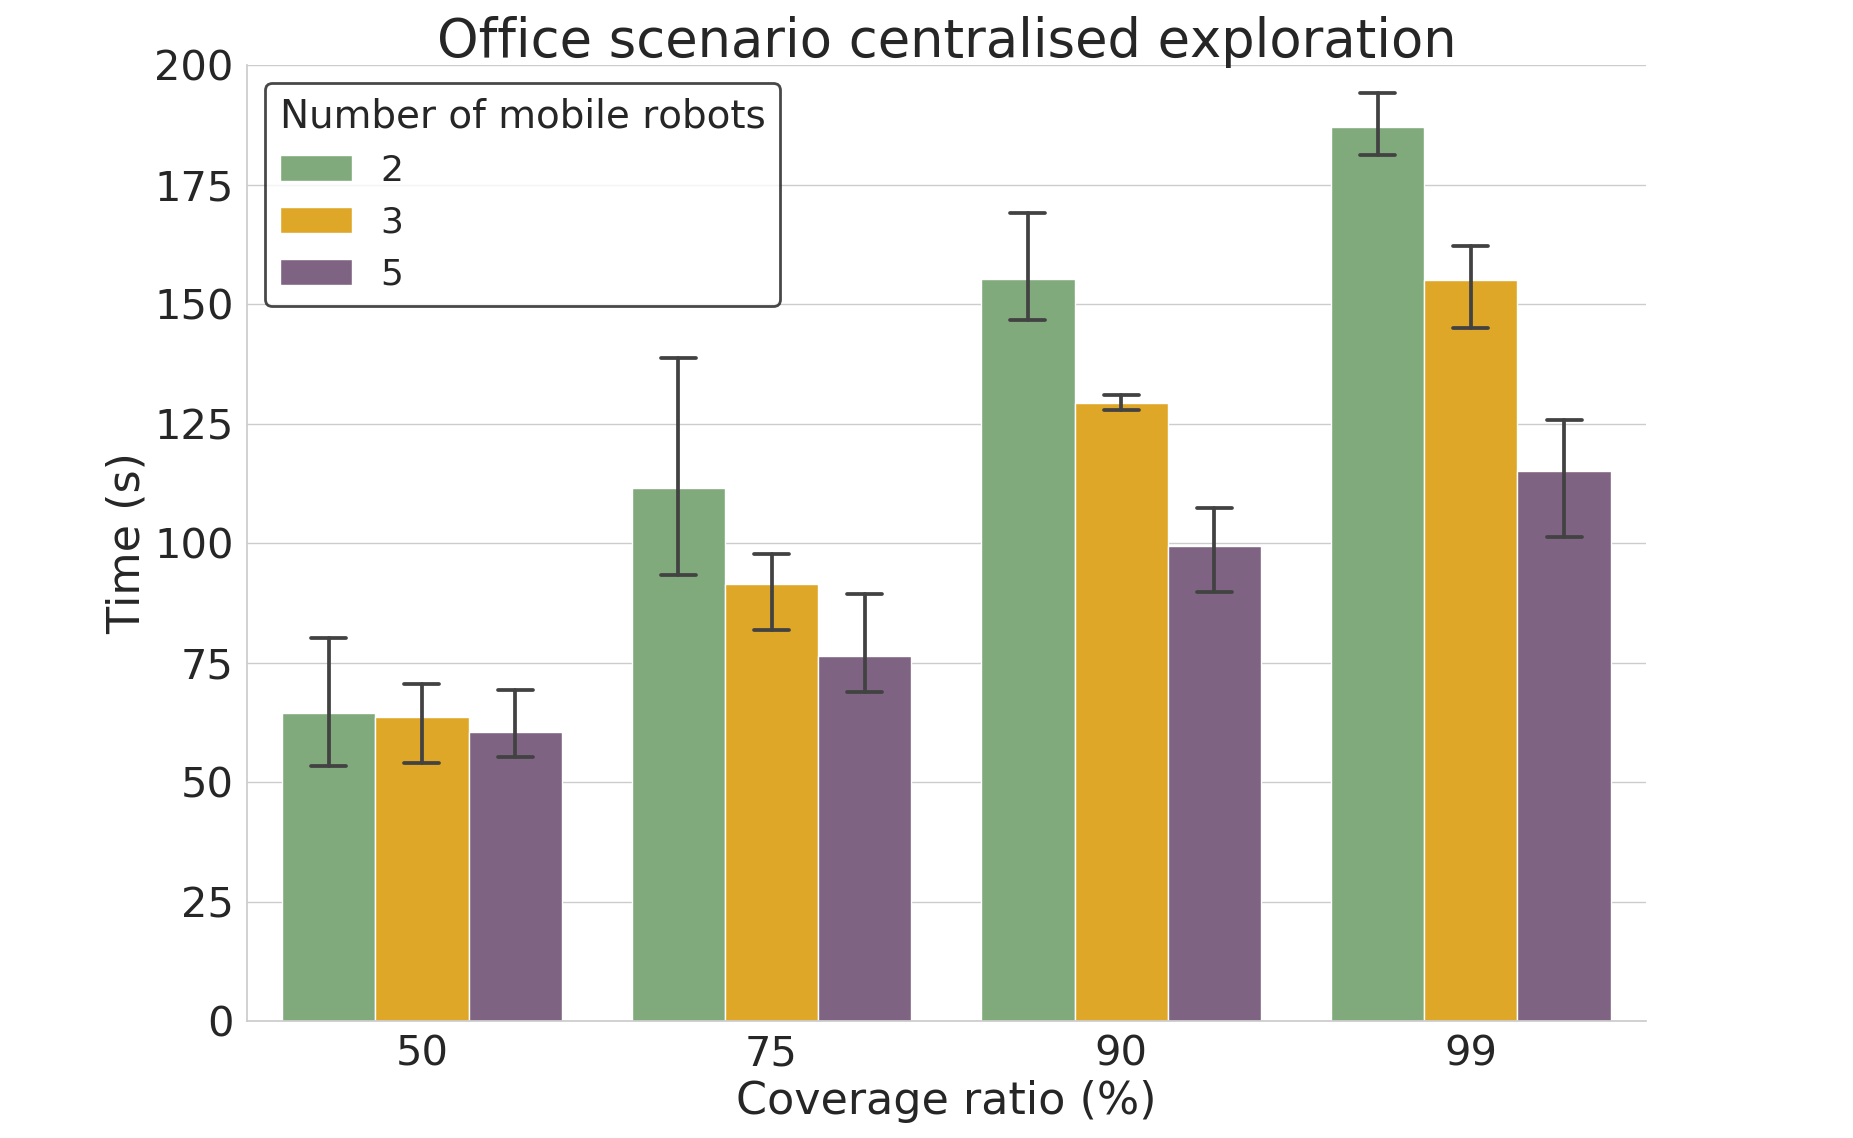
\includegraphics[width=0.46\textwidth]{office_c_cent.png}
        }\hfill
        \subfigure[\hspace{0.1cm} Coverage ratio over time in the office scenario for decentralised multi-robot exploration.]{%
           \label{fig:office_coverage_d}
           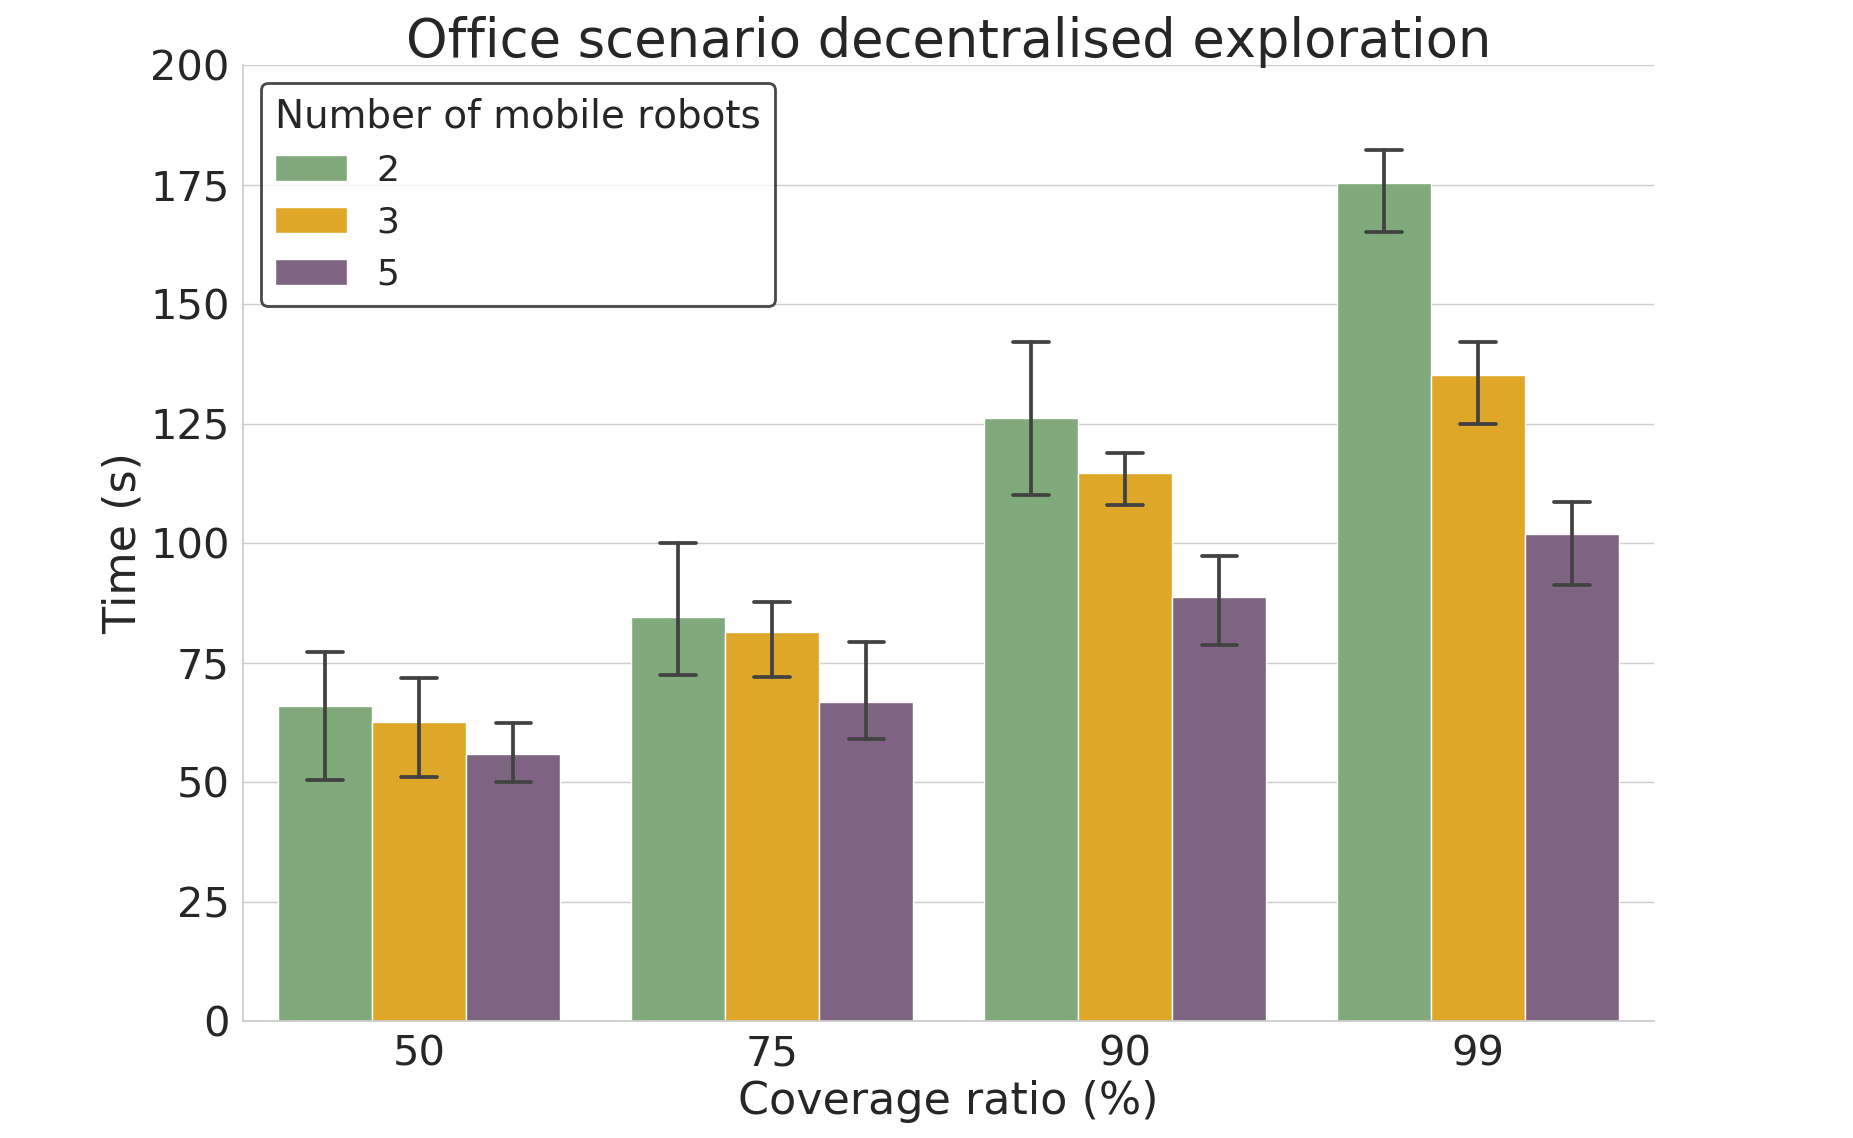
\includegraphics[width=0.46\textwidth]{office_c_decent.png}
        }\\ %  ------- End of the first row ----------------------%
        \subfigure[\hspace{0.1cm} Coverage ratio over time in the unstructured scenario for centralised multi-robot exploration.]{%
            \label{fig:unstruc_coverage_c}
            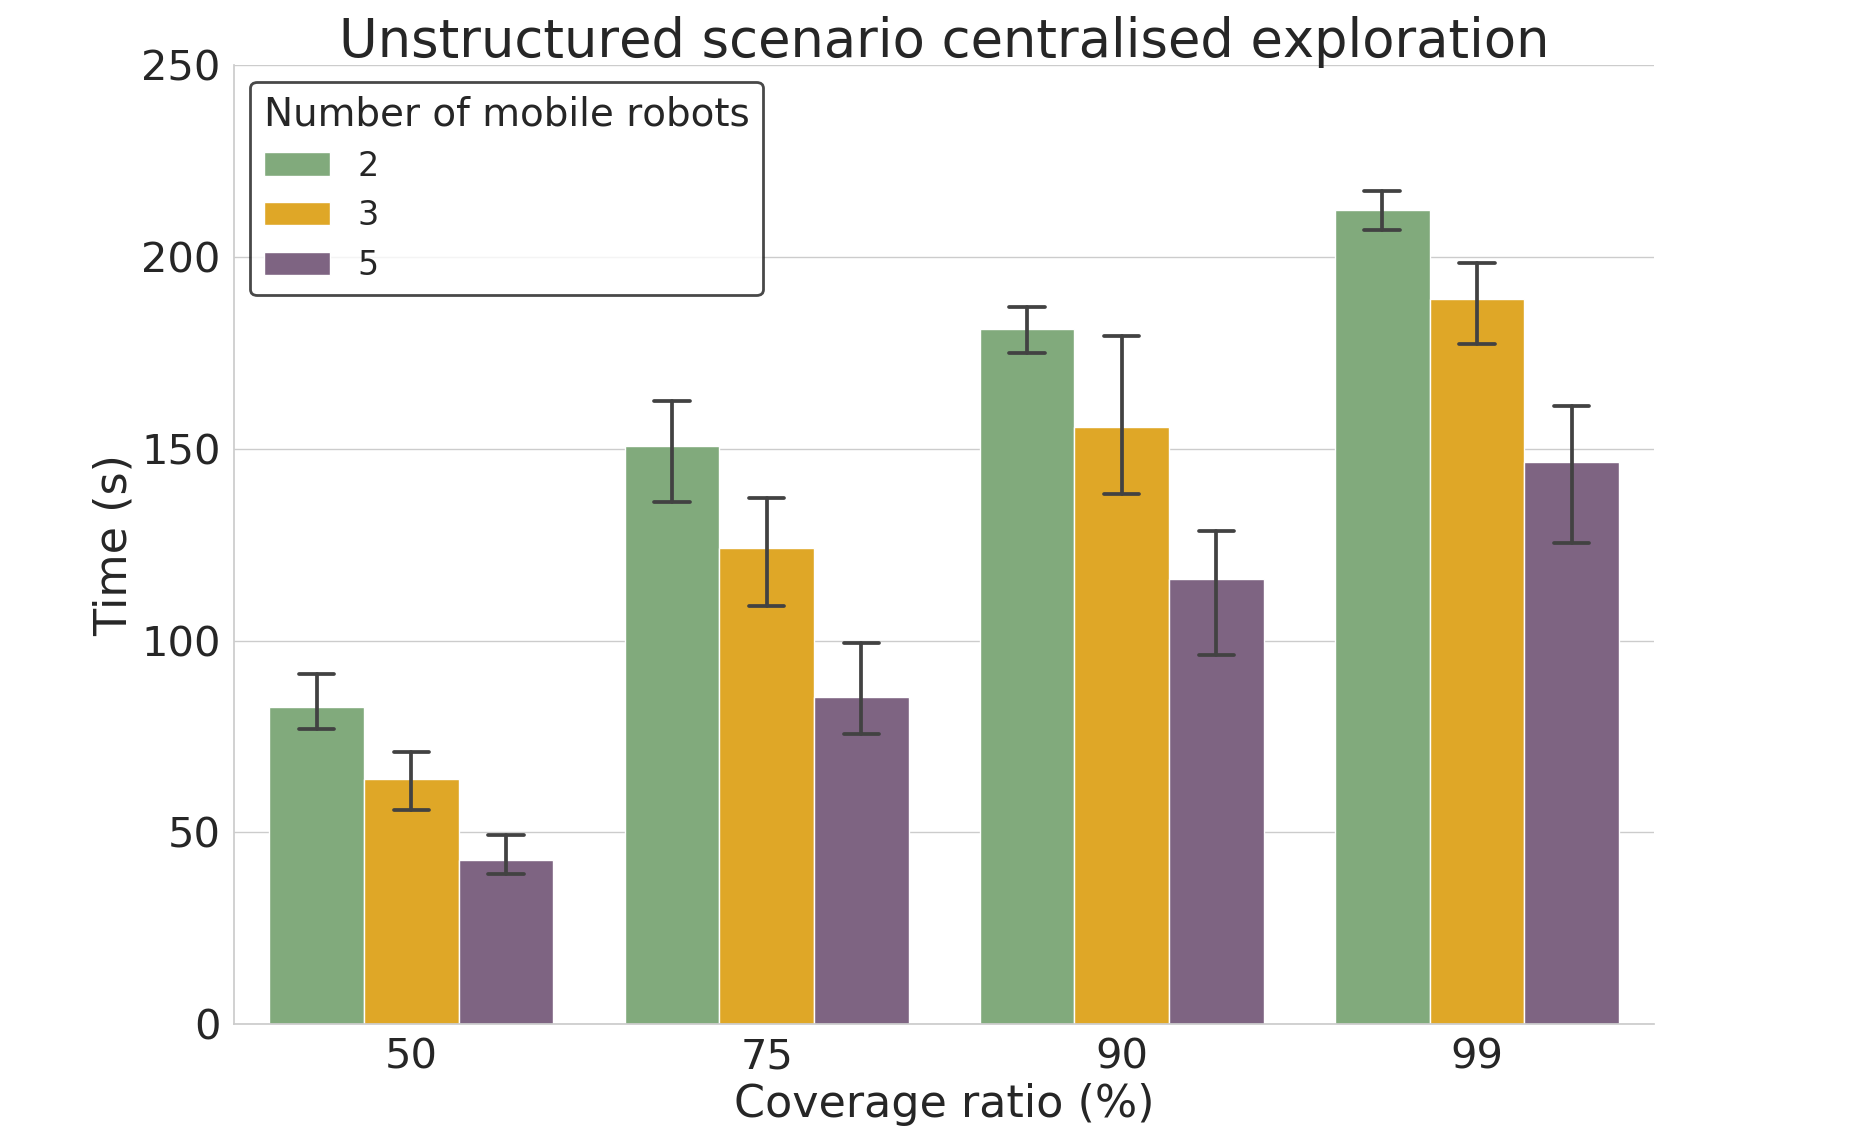
\includegraphics[width=0.46\textwidth]{unstructured_c_cent.png}
        }\hfill
        \subfigure[\hspace{0.1cm} Coverage ratio over time in the unstructured scenario for decentralised multi-robot exploration.]{%
            \label{fig:unstruc_coverage_d}
            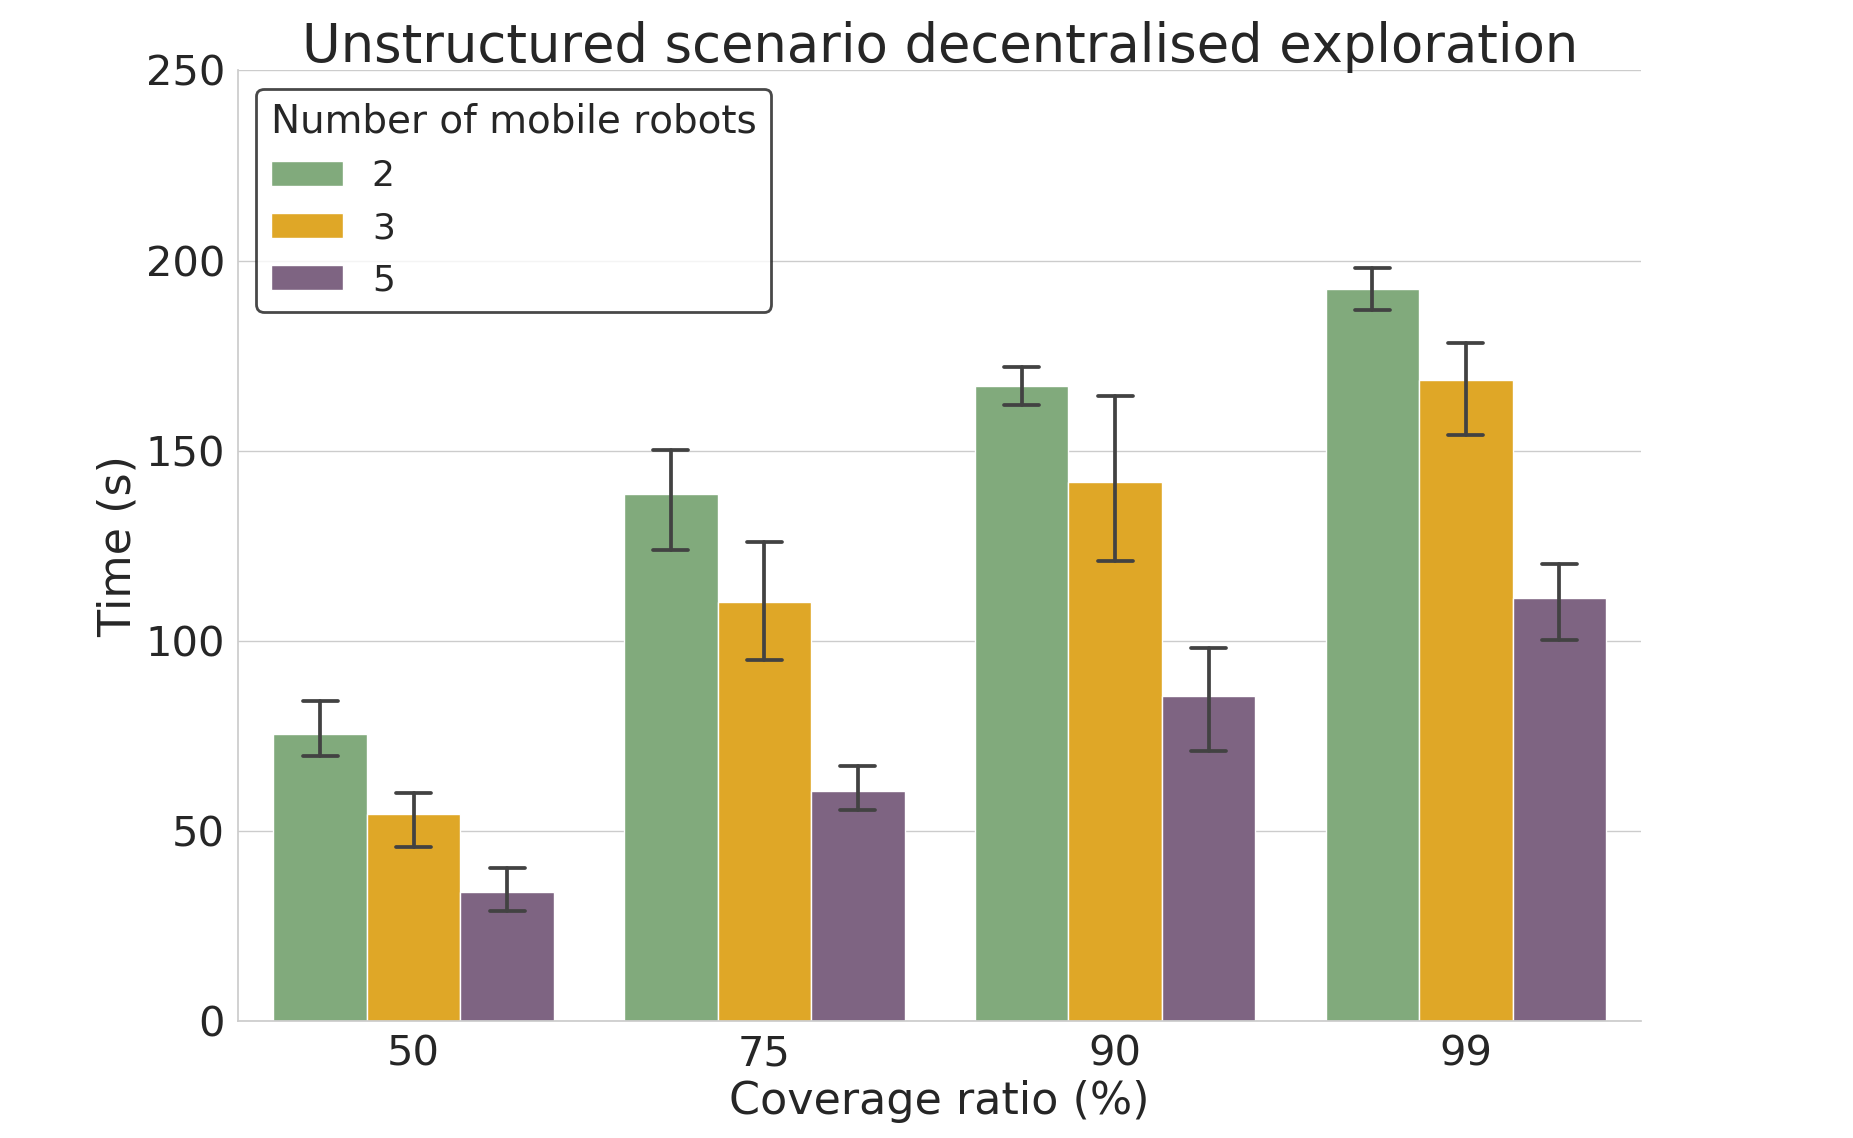
\includegraphics[width=0.46\textwidth]{unstructured_c_decent.png}
        }%
%
    \end{center}
    \caption{%
        The comparison of the coverage ratio over time during centralised and decentralised multi-robot exploration in the office scenario \subref{fig:office_coverage_c}, \subref{fig:office_coverage_d} and in the unstructured scenario \subref{fig:unstruc_coverage_c}, \subref{fig:unstruc_coverage_d}. 
     }%
   \label{fig:coverage_subfigures}
\end{figure*}

The frontier occupancy function $F_{ij}$ is the 2-dimensional Gaussian function with the position of the mean in a frontier point and with the standard deviation 
$3\sigma$= \begin{bmatrix}
           r_{f} \\
           r_{f} 
   \end{bmatrix}.
   
 If the frontier point $j$, for which the mobile robot $i$ is calculating the weight, is in the range of radius $r_{f}$ from the position of the mobile robot assigned point (\boldsymbol{q_{a}}); the value of the frontier occupancy function is calculated by Gaussian function, and zero otherwise (\ref{eq:frontier_funct}).

\begin{equation}\label{eq:frontier_funct}
 F_{ij}=
\begin{cases} 
       \lambda_{f} e^{-\Big[\frac{(q_{jx} - q_{ax})^2}{2\sigma_{x}^2} + \frac{(q_{jy} - q_{ay})^2}{2\sigma_{y}^2}\Big]} & \text{if $d(\boldsymbol{q_{j}}, \boldsymbol{q_{a}})< r_{f}$}, \\
      \quad \quad \quad \quad \quad 0 & \text{otherwise}
   \end{cases}
\end{equation}

where $\lambda_{f}$ is an experimentally determined constant. 

The function $F_{ij}$ is used to prevent assigning the frontier point to the mobile robot B if that point is close to a point already assigned to mobile robot A. The example of the frontier point $j$ and its radii $r$ and $r_{f}$ is shown in Fig. \ref{fig:radijusi}.

\begin{figure}[b!]
	\centering
	\fbox{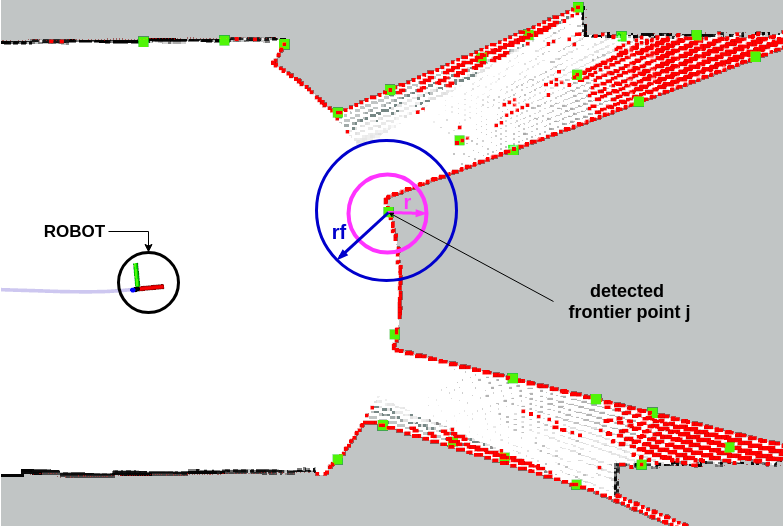
\includegraphics[width=0.85\columnwidth]{rviz_radius_vol4.png}}
	\caption{Detected frontier point $j$ and its radii $r$ and $r_{f}$.}
	\label{fig:radijusi}
\end{figure}

For each frontier point $j$, the weight $W_{ij}$ of the $i$-th mobile robot is calculated as: 
\begin{equation}
   {W}_{ij}= {C_{ij}} - {U_{ij}} + {F_{ij}}.
   \label{weight}
\end{equation}

The weight matrix $\boldsymbol{W}$ ($N\times M$) is formed for $N$ mobile robots and $M$ frontier points: 

\begin{equation}
    \boldsymbol{W} = \begin{bmatrix}
    W_{00} & W_{01} & \hdots & W_{0j} & \hdots & W_{0M}\\
    W_{10} & \ddots & & & & \vdots\\
    \vdots & & \ddots & & &  \vdots \\
    W_{i0} & & & \ddots & & \vdots \\
    \vdots & & & & \ddots & \vdots\\
    W_{N0} & \hdots  & \hdots  & \hdots  & \hdots &    W_{NM}
    \end{bmatrix}.
\end{equation}

The mobile robots exchange the information about weights for all frontier points and make decisions for the future actions based on the exchanged information. The amount of exchanged data is thus reduced, which allows for easier and faster communication.
The weight matrix $\boldsymbol{W}$ represents the input into the Hungarian algorithm that attempts to find an optimal assignment solution in polynomial time.

The Hungarian algorithm is described in \cite{Kuhn1955} and tested in \cite{Kulich2015}. Initially, the Hungarian algorithm assumes that the number of frontier points is the same as the number of mobile robots. Due to the fact that there are usually fewer mobile robots than frontier points, virtual mobile robots are added and then skipped during the process of assignment and exploration.

Let the matrix $X$ be the matrix of zeros and ones, where $X[i,j]=1$ iff the mobile robot $i$ is assigned to the frontier point $j$.
Than the optimal task assignment has weight:

\begin{equation}
     {\mathrm{min}}\ \sum_{i} \sum_{j} W_{ij}\ X_{ij},
\end{equation}

anticipating that minimisation of sum will ensure the dispersion of the mobile robots in the environment. 

\begin{algorithm}[H]
\caption{Decentralised strategy for mobile robot $i$}
\label{algorithm1}
\begin{algorithmic}[1]
\For{ each frontier point $j$}
\State\hspace{\algorithmicindent} $W_{ij}$ = $C_{ij}$ - $U_{ij}$ + $F_{ij}$
\State\hspace{\algorithmicindent} Send $W_{ij}$ to the other mobile robots.
\State \hspace{\algorithmicindent} Receive the weights from the others.
\State \hspace{\algorithmicindent} Calculate weight matrix $\boldsymbol{W}$.
\State \hspace{\algorithmicindent} Hungarian algorithm ($\boldsymbol{W}$).
\State{\textbf{return} Mobile robot $i$ is assigned to frontier point.}
\EndFor
\end{algorithmic}
\end{algorithm}

Our decentralised strategy executes during the robot motion and there are seven steps for each robot to be executed (Algorithm \ref{algorithm1}).  All frontier points are visible to every mobile robot.
When mobile robot $i$ is assigned to frontier point according to line 7 in Algorithm \ref{algorithm1}, the mobile robot starts to follow the planned path and navigate to the target frontier point. Moreover, at the moment when the mobile robot $i$ reaches the target point, a weight calculation request is sent to the other mobile robots, whose responses fill in the weight matrix $\boldsymbol{W}$ (which is an input to Hungarian algorithm). The described process executes until the whole environment is explored, in other words, until a complete  map of the environment is generated.
